%%%%%%%%%%%%%%%%%%%%%%%%%%%%%%%%%%%%%%%%%
% Beamer Presentation
% LaTeX Template
% Version 1.0 (10/11/12)
%
% This template has been downloaded from:
% http://www.LaTeXTemplates.com
%
% License:
% CC BY-NC-SA 3.0 (http://creativecommons.org/licenses/by-nc-sa/3.0/)
%
%%%%%%%%%%%%%%%%%%%%%%%%%%%%%%%%%%%%%%%%%

%----------------------------------------------------------------------------------------
%	PACKAGES AND THEMES
%----------------------------------------------------------------------------------------

\documentclass[UTF8,aspectratio=169,14pt]{ctexbeamer}

\usepackage{hyperref}
\hypersetup{
	colorlinks=true,
	linkcolor=red,
	anchorcolor=blue,
	citecolor=green
}

\mode<presentation> {
	
	% The Beamer class comes with a number of default slide themes
	% which change the colors and layouts of slides. Below this is a list
	% of all the themes, uncomment each in turn to see what they look like.
	
	%\usetheme{default}
	%\usetheme{AnnArbor}
	%\usetheme{Antibes}
	%\usetheme{Bergen}
	%\usetheme{Berkeley}
	%\usetheme{Berlin}
	%\usetheme{Boadilla}
	%\usetheme{CambridgeUS}
	%\usetheme{Copenhagen}
	%\usetheme{Darmstadt}
	%\usetheme{Dresden}
	%\usetheme{Frankfurt}
	%\usetheme{Goettingen}
	%\usetheme{Hannover}
	%\usetheme{Ilmenau}
	%\usetheme{JuanLesPins}
	%\usetheme{Luebeck}
	\usetheme{Madrid}
	%\usetheme{Malmoe}
	%\usetheme{Marburg}
	%\usetheme{Montpellier}
	%\usetheme{PaloAlto}
	%\usetheme{Pittsburgh}
	%\usetheme{Rochester}
	%\usetheme{Singapore}
	%\usetheme{Szeged}
	%\usetheme{Warsaw}
	
	% As well as themes, the Beamer class has a number of color themes
	% for any slide theme. Uncomment each of these in turn to see how it
	% changes the colors of your current slide theme.
	
	%\usecolortheme{albatross}
	%\usecolortheme{beaver}
	%\usecolortheme{beetle}
	%\usecolortheme{crane}
	%\usecolortheme{dolphin}
	%\usecolortheme{dove}
	%\usecolortheme{fly}
	%\usecolortheme{lily}
	%\usecolortheme{orchid}
	%\usecolortheme{rose}
	%\usecolortheme{seagull}
	%\usecolortheme{seahorse}
	%\usecolortheme{whale}
	%\usecolortheme{wolverine}
	
	%\setbeamertemplate{footline} % To remove the footer line in all slides uncomment this line
	%\setbeamertemplate{footline}[page number] % To replace the footer line in all slides with a simple slide count uncomment this line
	
	%\setbeamertemplate{navigation symbols}{} % To remove the navigation symbols from the bottom of all slides uncomment this line
}

\usepackage{graphicx} % Allows including images
\graphicspath{{./figs/}}
\usepackage{booktabs} % Allows the use of \toprule, \midrule and \bottomrule in tables
\usepackage{longtable}
\usepackage{listings}
\usepackage{xcolor}
\lstset{numbers=left, %设置行号位置
	numberstyle=\tiny, %设置行号大小
	keywordstyle=\color{blue}, %设置关键字颜色
	commentstyle=\color[cmyk]{1,0,1,0}, %设置注释颜色
	frame=single, %设置边框格式
	escapeinside=``, %逃逸字符(1左面的键),用于显示中文
	%breaklines, %自动折行
	extendedchars=false, %解决代码跨页时,章节标题,页眉等汉字不显示的问题
	xleftmargin=2em,xrightmargin=2em, aboveskip=1em, %设置边距
	tabsize=4, %设置tab空格数
	showspaces=false %不显示空格
}
% Fonts
% \usepackage{libertine}
% \setmonofont{Courier}
\setCJKsansfont[ItalicFont=Noto Serif CJK SC Black, BoldFont=Noto Sans CJK SC Black]{Noto Sans CJK SC}

%\def\imagepath{./resources/graphics}
%\usepackage[imagepath=\imagepath]{ditaa}
%\graphicspath{ {\imagepath/} }


%\usepackage{pgfpages}
%\setbeameroption{show notes on second screen}
%%----------------------------------------------------------------------------------------
%	TITLE PAGE
%----------------------------------------------------------------------------------------

\title[第10讲]{第十一讲:处理机调度} % The short title appears at the bottom of every slide, the full title is only on the title page
\subtitle{第7节:rCore调度框架}
\author{向勇、陈渝} % Your name
\institute[清华大学] % Your institution as it will appear on the bottom of every slide, may be shorthand to save space
{
	清华大学计算机系 \\ % Your institution for the title page
	\medskip
	\textit{xyong,yuchen@tsinghua.edu.cn} % Your email address
}
\date{\today} % Date, can be changed to a custom date


\begin{document}
%----------------------------------------------
\begin{frame}
\titlepage % Print the title page as the first slide
\end{frame}
%----------------------------------------------
\begin{frame}
\frametitle{提纲} % Table of contents slide, comment this block out to remove it
\tableofcontents % Throughout your presentation, if you choose to use \section{} and \subsection{} commands, these will automatically be printed on this slide as an overview of your presentation
\end{frame}
%----------------------------------------------
%%	PRESENTATION SLIDES
%----------------------------------------------
%------------------------------------------------
\section{第7节:rCore调度框架}% Sections can be created in order to organize your presentation into discrete blocks, all sections and subsections are automatically printed in the table of contents as an overview of the talk
%------------------------------------------------
\subsection{调度框架} % A subsection can be created just before a set of slides with a common theme to further break down your presentation into chunks
%------------------------------------------------
\begin{frame}[fragile]
    \frametitle{rCore调度框架}
    \subframetitle{rcore-thread/src/scheduler/mod.rs}
%% figure
    \begin{figure}
    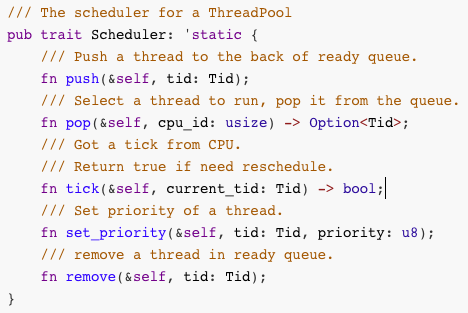
\includegraphics[width=0.65\linewidth]{figs/Scheduler.png}
%    \caption{xxxx}
    \end{figure}
\end{frame}
%------------------------------------------------
% ### 11.7 rCore调度框架和时间片轮转调度算法
% 
% #### 调度框架与线程控制
% /Users/xyong/github/rcore-thread/src/scheduler/mod.rs
% pub trait Scheduler: 'static
% 
% ![Scheduler](/Users/xyong/Desktop/figs/Scheduler.png)
% 
% ```rust
% /// The scheduler for a ThreadPool
% pub trait Scheduler: 'static {
%     /// Push a thread to the back of ready queue.
%     fn push(&self, tid: Tid);
%     /// Select a thread to run, pop it from the queue.
%     fn pop(&self, cpu_id: usize) -> Option<Tid>;
%     /// Got a tick from CPU.
%     /// Return true if need reschedule.
%     fn tick(&self, current_tid: Tid) -> bool;
%     /// Set priority of a thread.
%     fn set_priority(&self, tid: Tid, priority: u8);
%     /// remove a thread in ready queue.
%     fn remove(&self, tid: Tid);
% }
% ```
% 
%------------------------------------------------
\begin{frame}[fragile]
    \frametitle{与调度相关的线程控制函数}
    \subframetitle{rcore-thread/src/thread\_pool.rs}
%% figure
    \begin{figure}
    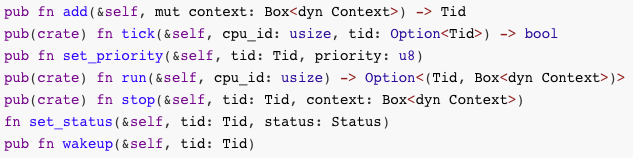
\includegraphics[width=1.0\linewidth]{figs/thread-pool-scheduler.png}
%    \caption{xxxx}
    \end{figure}
\end{frame}
%------------------------------------------------
% /Users/xyong/github/rcore-thread/src/thread_pool.rs
% self.scheduler.
% 与调度相关的线程控制函数
% 
% ![thread-pool-scheduler](/Users/xyong/Desktop/figs/thread-pool-scheduler.png)
% 
% ```rust
% pub fn add(&self, mut context: Box<dyn Context>) -> Tid
% pub(crate) fn tick(&self, cpu_id: usize, tid: Option<Tid>) -> bool
% pub fn set_priority(&self, tid: Tid, priority: u8)
% pub(crate) fn run(&self, cpu_id: usize) -> Option<(Tid, Box<dyn Context>)>
% pub(crate) fn stop(&self, tid: Tid, context: Box<dyn Context>)
% fn set_status(&self, tid: Tid, status: Status)
% pub fn wakeup(&self, tid: Tid)
% ```
%------------------------------------------------
%\subsection{调度数据结构} % A subsection can be created just before a set of slides with a common theme to further break down your presentation into chunks
%------------------------------------------------
\begin{frame}[fragile]
    \frametitle{调度数据结构:struct ThreadPool}
%    \subframetitle{struct ThreadPool}
    \subframetitle{rcore-thread/src/thread\_pool.rs}
%% figure
\begin{figure}
    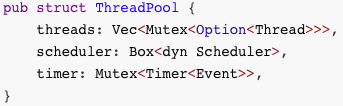
\includegraphics[width=0.55\linewidth]{figs/ThreadPool.png}
%    \caption{xxxx}
    \end{figure}
\end{frame}
%------------------------------------------------
% #### 调度数据结构
% 
% /Users/xyong/github/rcore-thread/src/scheduler/mod.rs
% pub trait Scheduler: 'static
% 调度算法接口
% 
% /Users/xyong/github/rcore-thread/src/thread_pool.rs
% pub struct ThreadPool
% 线程池数据结构
% 记录调度算法相关信息和参数;
% 
% ![ThreadPool](/Users/xyong/Desktop/figs/ThreadPool.png)
% 
% ```rust 
% pub struct ThreadPool {
%     threads: Vec<Mutex<Option<Thread>>>,
%     scheduler: Box<dyn Scheduler>,
%     timer: Mutex<Timer<Event>>,
% }
% ```
% 
%------------------------------------------------
\begin{frame}[fragile]
    \frametitle{调度算法和参数设置}
%    \framesubtitle{调度算法和参数设置}
    \subframetitle{rCore/kernel/src/process/mod.rs}
%% figure
\begin{figure}
    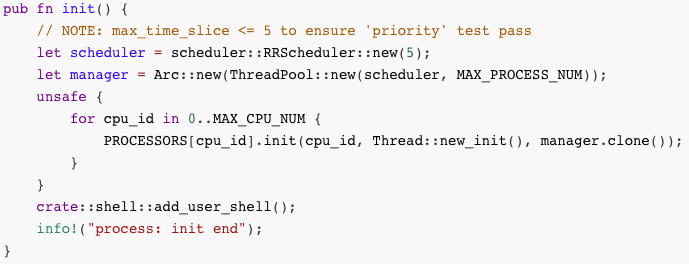
\includegraphics[width=0.9\linewidth]{figs/scheduler-init.png}
%    \caption{xxxx}
    \end{figure}
\end{frame}
% /Users/xyong/github/rCore/kernel/src/process/mod.rs
% pub fn init()
% 初始化函数
% 指定调度算法;
% 初始化线程池;
% 
% ![scheduler-init](/Users/xyong/Desktop/figs/scheduler-init.png)
% 
% ```rust
% pub fn init() {
%     // NOTE: max_time_slice <= 5 to ensure 'priority' test pass
%     let scheduler = scheduler::RRScheduler::new(5);
%     let manager = Arc::new(ThreadPool::new(scheduler, MAX_PROCESS_NUM));
%     unsafe {
%         for cpu_id in 0..MAX_CPU_NUM {
%             PROCESSORS[cpu_id].init(cpu_id, Thread::new_init(), manager.clone());
%         }
%     }
%     crate::shell::add_user_shell();
%     info!("process: init end");
% }
% ```
% 
%------------------------------------------------
\subsection{时间片轮转(Round Robin)调度算法} % A subsection can be created just before a set of slides with a common theme to further break down your presentation into chunks
%------------------------------------------------
\begin{frame}[fragile]
    \frametitle{时间片轮转(Round Robin)调度算法:数据结构}
    \subframetitle{rcore-thread/src/scheduler/rr.rs}
%% figure
    \begin{figure}
    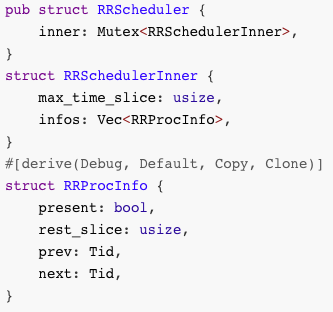
\includegraphics[width=0.45\linewidth]{figs/RRScheduler.png}
%    \caption{xxxx}
    \end{figure}
\end{frame}
%------------------------------------------------

% #### 时间片轮转调度算法
% 
% /Users/xyong/github/rcore-thread/src/scheduler/rr.rs
% pub struct RRScheduler RR调度算法数据结构
% struct RRSchedulerInner 线程双向链表表头数据结构
% struct RRProcInfo 线程双向链表节点数据结构
% 
% ![RRScheduler](/Users/xyong/Desktop/figs/RRScheduler.png)
% 
% ```rust
% pub struct RRScheduler {
%     inner: Mutex<RRSchedulerInner>,
% }
% struct RRSchedulerInner {
%     max_time_slice: usize,
%     infos: Vec<RRProcInfo>,
% }
% #[derive(Debug, Default, Copy, Clone)]
% struct RRProcInfo {
%     present: bool,
%     rest_slice: usize,
%     prev: Tid,
%     next: Tid,
% }
% ```
%------------------------------------------------
\begin{frame}[fragile]
    \frametitle{RR调度算法实现}
%    \framesubtitle{yyyy}
%% figure
    \begin{figure}
    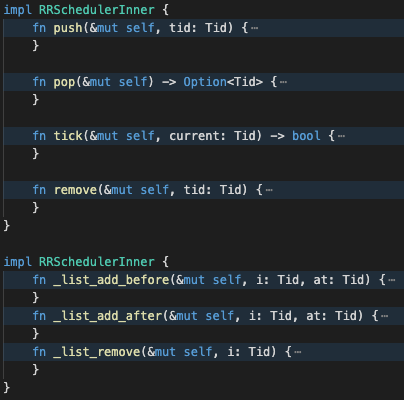
\includegraphics[width=0.45\linewidth]{figs/RRSchedulerInner.png}
%    \caption{xxxx}
    \end{figure}
\end{frame}
% impl RRSchedulerInner
% 具体的调度接口实现函数
% 
% ![RRSchedulerInner](/Users/xyong/Desktop/figs/RRSchedulerInner.png)
% 
% 
%------------------------------------------------
%\subsection{线程调度和切换过程} % A subsection can be created just before a set of slides with a common theme to further break down your presentation into chunks
%------------------------------------------------
\begin{frame}[fragile]
    \frametitle{时间片用完时的线程调度和切换过程}
%    \framesubtitle{yyyy}
%% figure
    \begin{figure}
    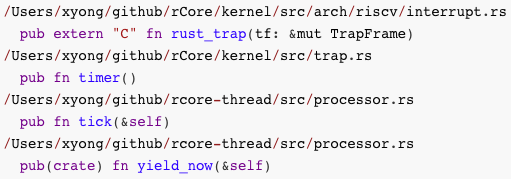
\includegraphics[width=0.8\linewidth]{figs/RR-timeout.png}
%    \caption{xxxx}
    \end{figure}
\end{frame}
%------------------------------------------------
% #### 时间片用完时的线程调度和切换过程
% 
% /Users/xyong/github/rCore/kernel/src/arch/riscv/interrupt.rs
% pub extern "C" fn rust_trap(tf: &mut TrapFrame)
% Trap::Interrupt(I::SupervisorTimer) => timer(),
% 
% /Users/xyong/github/rCore/kernel/src/trap.rs
% pub fn timer()
% processor().tick();
% 
% /Users/xyong/github/rcore-thread/src/processor.rs
% pub fn tick(&self)
% let need_reschedule = self.manager().tick(self.inner().id, tid);
% 
% /Users/xyong/github/rcore-thread/src/processor.rs
% pub(crate) fn yield_now(&self)
% .switch_to(&mut *inner.loop_context);
% 
% ```rust
% /Users/xyong/github/rCore/kernel/src/arch/riscv/interrupt.rs
%   pub extern "C" fn rust_trap(tf: &mut TrapFrame)
% /Users/xyong/github/rCore/kernel/src/trap.rs
%   pub fn timer()
% /Users/xyong/github/rcore-thread/src/processor.rs
%   pub fn tick(&self)
% /Users/xyong/github/rcore-thread/src/processor.rs
%   pub(crate) fn yield_now(&self)
% ```
%------------------------------------------------
\end{document}
